\documentclass[12pt,notitlepage]{article}
\usepackage[bitstream-charter]{mathdesign}
\usepackage{inconsolata}
\usepackage[T1]{fontenc}
\usepackage{microtype}
\usepackage{graphicx}
\usepackage[utf8x]{inputenc}
\usepackage[letterpaper]{geometry}

\begin{document}
\title{Proposal: Concreteness Fading and Visual Programming in
  Teaching Object-Oriented Programming}
\author{Andy Jiang, Michael Mauer, and David Li}

\maketitle

Much effort has gone towards methods to teach programming as an
overall concept, with systems like Alice, Scratch, and CodeSpells
demonstrating how visual programming can successfully introduce
students to this field. Our goal is to teach the more specific topic
of object-oriented programming to novice programmers using these same
techniques, focusing on how to abstract and represent ideas such as
inheritance, polymorphism, and interfaces in such a
framework. Additionally, to reinforce these concepts to an audience
already somewhat familiar with programming, we will introduce
concreteness fading to the system, transitioning students from visual
programming to directly writing code. This will facilitate the
learning of specific higher-level concepts and abstractions within
computer science, which is important to effectively educate and train
the next generation of computer science and software development
students.

Our approach is to develop a game involving visual programming, where
the objective is to manipulate various objects within a world to
accomplish certain goals. Tentatively, the main theme will be
controlling a robot. Students will control the robot and other objects
via a block-based visual programming interface akin to
Scratch. However, the interface will be oriented towards expressing
object-oriented concepts, making clear ideas such as method
invocation, object instantiation, and polymorphism. Furthermore, the
intent is to demonstrate the link between the abstracted
representation and the underlying code: the system will translate the
visual representation to Java code, showing its execution in tandem
with the symbolic execution of the blocks and the effect of the code
in the world. Eventually, the system will fade the visual
representation, asking students to directly write more and more of the
code itself.

\begin{figure}[h]
  \centering
  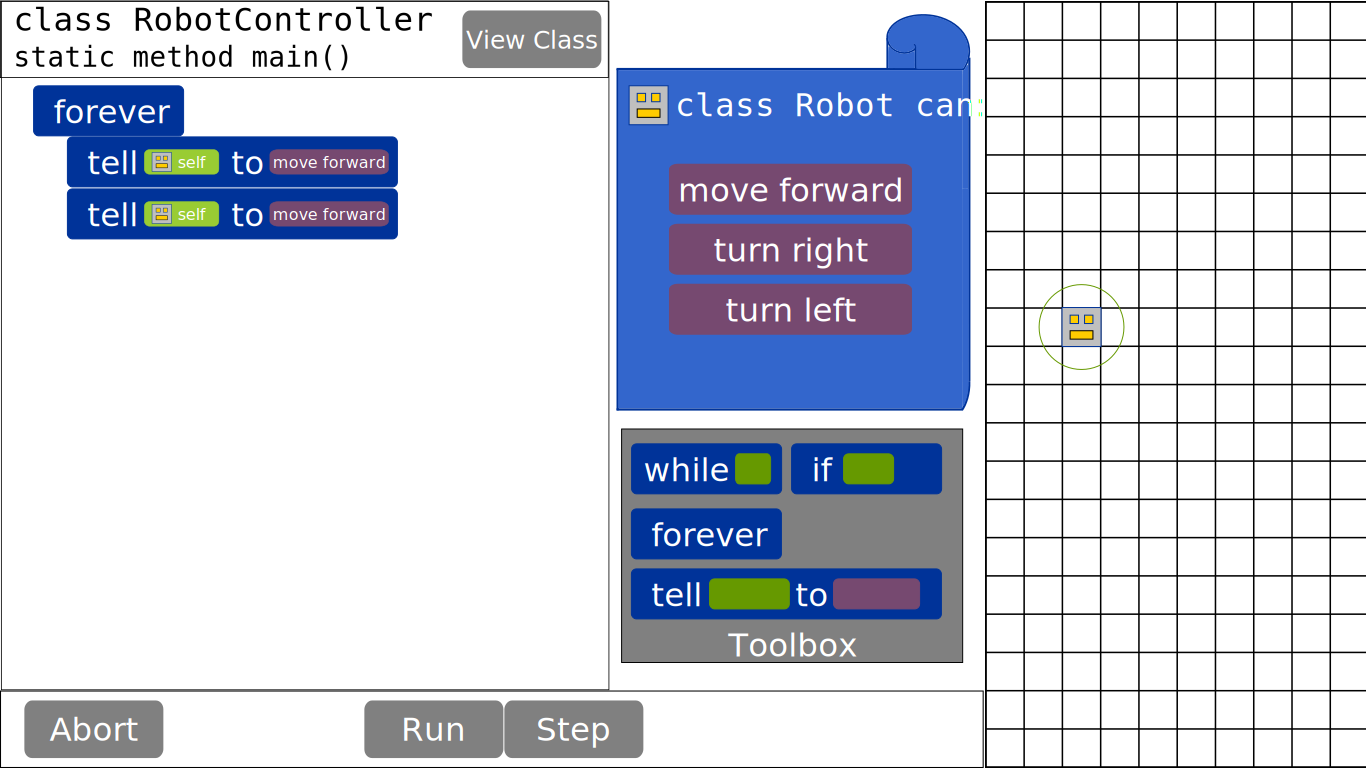
\includegraphics[width=\textwidth]{mockup.pdf}
  \caption{The main game interface.}
\end{figure}

\end{document}
